\documentclass[tikz,border=2]{standalone}
\usetikzlibrary{shadows,arrows,shapes,positioning,calc,backgrounds,fit}
\newcommand{\vanish}[1]{}
\usepackage{colortbl}
\usepackage{array}
\usepackage{multirow}
\newcommand{\shaded}[1]{\cellcolor{black!20}{#1}}
\newcommand{\calc}[1]{\mbox{$\mathcal{C}_{#1}$}}
\pdfpageattr {/Group << /S /Transparency /I true /CS /DeviceRGB>>}
% Define the layers to draw the diagram
%
\begin{document}
%% \pgfdeclarelayer{bg}
%% \pgfdeclarelayer{fg}
%% \pgfsetlayers{bg,main,fg}
%
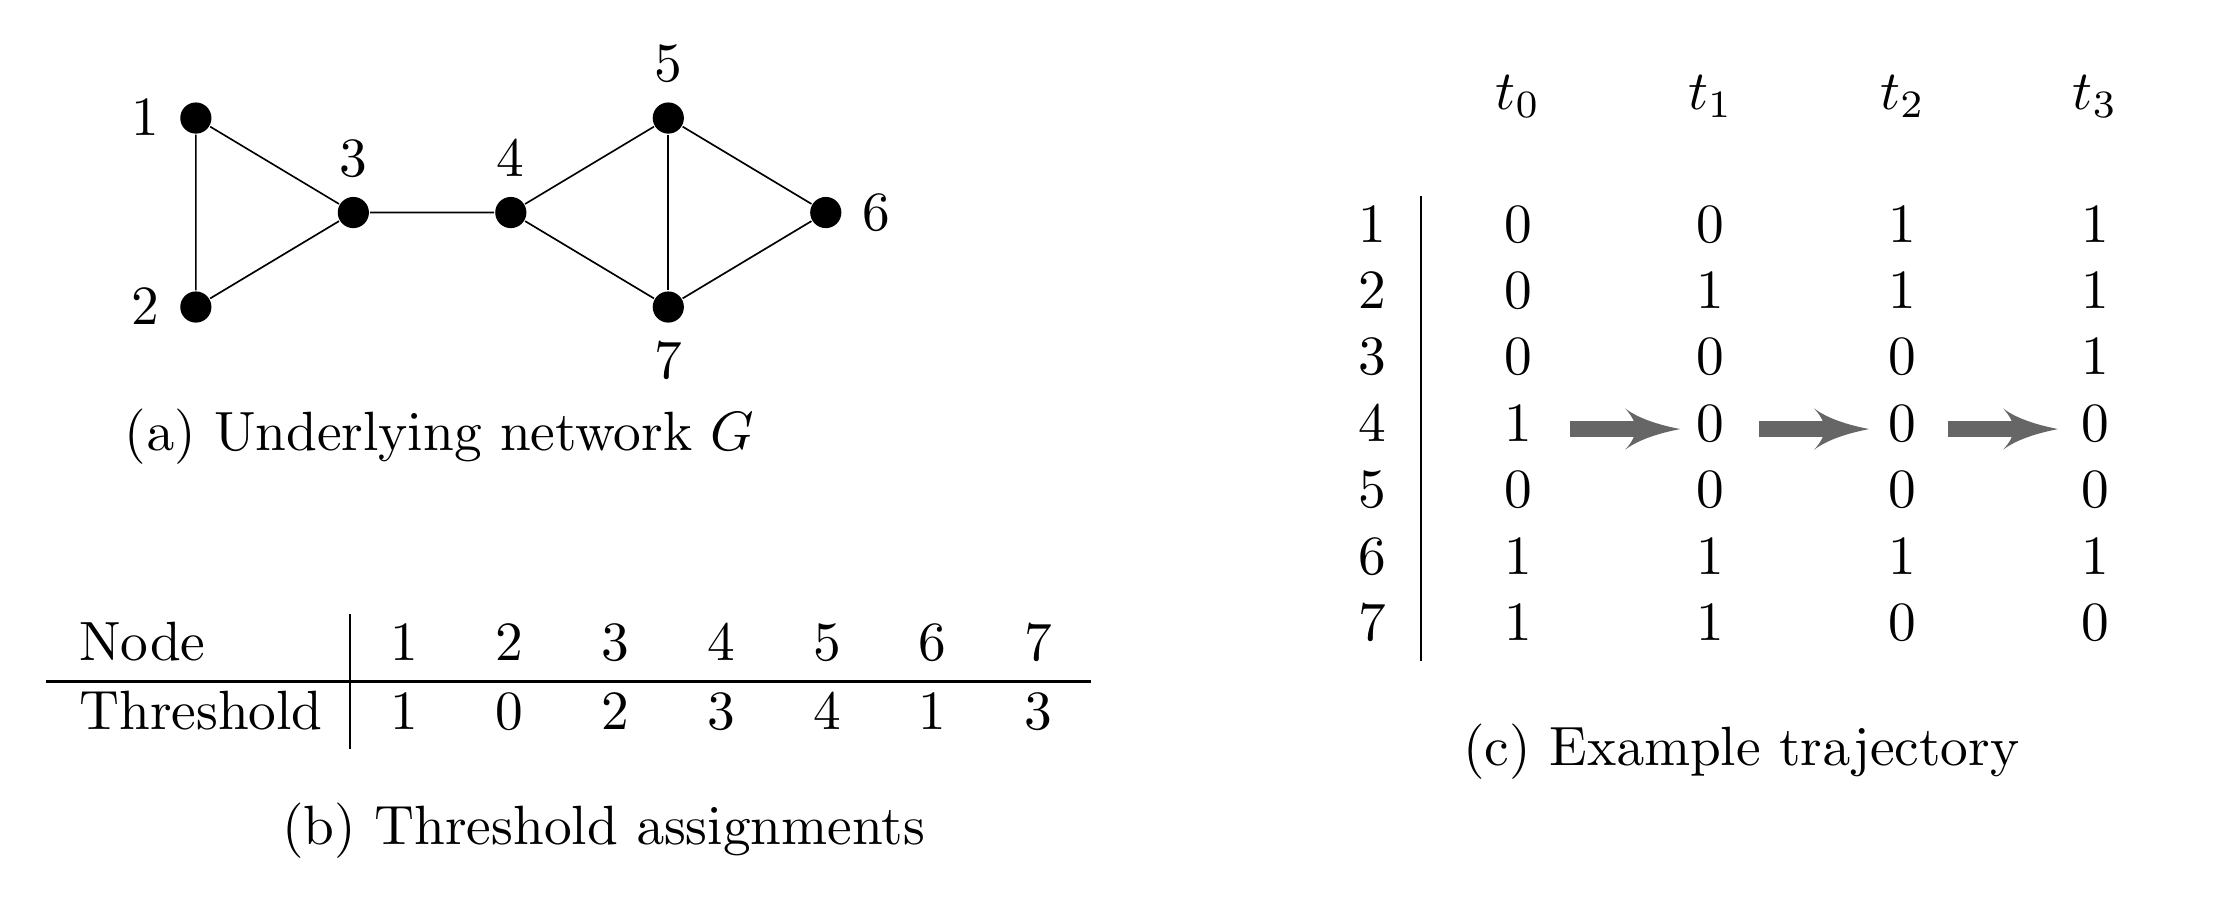
\begin{tikzpicture}
[scale=2,node distance=.5cm, transform shape,
    vertex/.style={shape=circle,fill,inner sep=.7mm},
myblock/.style={draw=none,fill=none,scale=1.5,inner sep=0pt},
myedge/.style={>=latex', shorten >=.0pt, shorten <=.0pt,semithick},
diredge/.style={>=latex', shorten >=.0pt, shorten <=.0pt,line
width=2mm,black!60},
every fit/.style={fill=black!10,ellipse,draw=black!20},
myellipse/.style={fill=black!20,draw=none}]
%%%%%%%%%%
%%%%% The underlying graph
\begin{scope}[anchor=north west,shift={(0.5,0)}]
\node (v1) [vertex,label=left:$1$] at (0,.6) {};
\node (v2) [vertex,label=left:$2$] at (0,-.6) {};
\node (v3) [vertex,label=above:$3$] at (1,0) {};
\node (v4) [vertex,label=above:$4$] at (2,0) {};
\node (v5) [vertex,label=above:$5$] at (3,.6) {};
\node (v6) [vertex,label=right:$6$] at (4,0) {};
\node (v7) [vertex,label=below:$7$] at (3,-.6) {};
\path[draw,myedge] (v1) -- (v2) -- (v3) -- (v4) -- (v5) -- (v6) --
(v7) -- (v4);
\path[draw,myedge] (v1) -- (v3);
\path[draw,myedge] (v5) -- (v7);
\node[anchor=west] at (-.5,-1.5) {(a) Underlying network $G$};
\end{scope}
%%
%%%%% thresholds and colors
\begin{scope}[anchor=north west,shift={(-.5,-2.5)}]
\node [draw=none, fill=none, shape=rectangle,scale=1] at (0,0) {
   \begin{tabular}{p{15mm}|>{\centering\arraybackslash}p{2.5mm}>{\centering\arraybackslash}p{2.5mm}>{\centering\arraybackslash}p{2.5mm}>{\centering\arraybackslash}p{2.5mm}>{\centering\arraybackslash}p{2.5mm}>{\centering\arraybackslash}p{2.5mm}>{\centering\arraybackslash}p{2.5mm}}
Node    & $1$ & $2$ & $3$ & $4$ & $5$ & $6$ & $7$ \\\hline
Threshold & $1$ & $0$ & $2$ & $3$ & $4$ & $1$ & $3$ 
    \end{tabular}
};
\node [anchor=west] at (1.5,-1.5) {(b) Threshold assignments};
\end{scope}
%%
%%%%% example trajectory
\begin{scope}[anchor=north west,shift={(7.5,1)}]
\node [anchor=north west,draw=none, fill=none, shape=rectangle,scale=1] at (0,0) {
    \begin{tabular}{>{\hfill}p{3mm}|>{\centering\arraybackslash}p{8mm}>{\centering\arraybackslash}p{8mm}>{\centering\arraybackslash}p{8mm}>{\centering\arraybackslash}p{8mm}}
\multicolumn{1}{r}{} & $t_0$ & $t_1$ & $t_2$ & $t_3$ \\
\multicolumn{1}{r}{} & & & & \\
1 & $0$ & $0$ & $1$ & $1$ \\
2 & $0$ & $1$ & $1$ & $1$ \\
3 & $0$ & $0$ & $0$ & $1$ \\
4 & $1$ & $0$ & $0$ & $0$ \\
5 & $0$ & $0$ & $0$ & $0$ \\
6 & $1$ & $1$ & $1$ & $1$ \\
7 & $1$ & $1$ & $0$ & $0$
\end{tabular}
};

\draw[diredge,->] (1.8,-2.45) -- +(.7,0);
\draw[diredge,->] (3.0,-2.45) -- +(.7,0);
\draw[diredge,->] (4.2,-2.45) -- +(.7,0);
\node [anchor=west] at (1,-4.5) {(c) Example trajectory};
\end{scope}
%%
\end{tikzpicture}
\end{document}
